% siminos/kittens/Bernoulli.tex      pdflatex CL18
% $Author: predrag $ $Date: 2021-05-07 11:35:26 -0400 (Fri, 07 May 2021) $

\section{A fair coin toss}
\label{s:coinToss}
\renewcommand{\ssp}{\ensuremath{x}}               % state space point

The very simplest example of a deterministic law of evolution that gives
rise to `chaos' is the {\em Bernoulli} map, \reffig{fig:BernPart}\,(a),
which models a
\HREF{https://www.random.org/coins/?num=2&cur=40-antique.aurelian} {coin
toss}. Starting with a random initial state, the map generates,
deterministically,  a sequence of tails and heads with the 50-50\%
probability.

We introduce the model in its conventional, time-evolution dynamical
formulation, than reformulate it as a lattice `field theory', solved by
enumeration of all admissible \emph{lattice states}, field configurations that
satisfy a  global fixed point condition, and use this simple setting to
motivate (1) the \emph{fundamental fact}: for a given lattice period,
the {\em \HillDet} of stabilities of
global solutions counts their number, and (2) the
{\tzeta} counts their symmetry orbits, with a \emph{prime} lattice state per
each orbit.

\subsection{Bernoulli map} %Doubling map}
\label{s:Bernoulli}
%ChaosBook return to
% \example{Bernoulli shift map \statesp\ partition.}{ \label{exam:BernMap}

\renewcommand{\statesp}{state space}
\renewcommand{\Statesp}{State space}
\renewcommand{\stateDsp}{state-space}
\renewcommand{\StateDsp}{State-space}

%
%%%%%%%%%%%%%%%%%%%%%%%%%%%%%%%%%%%%%%%%%%%%%%%%%%%%%%%%%%%%%
\begin{figure}
  \centering
{(a)}
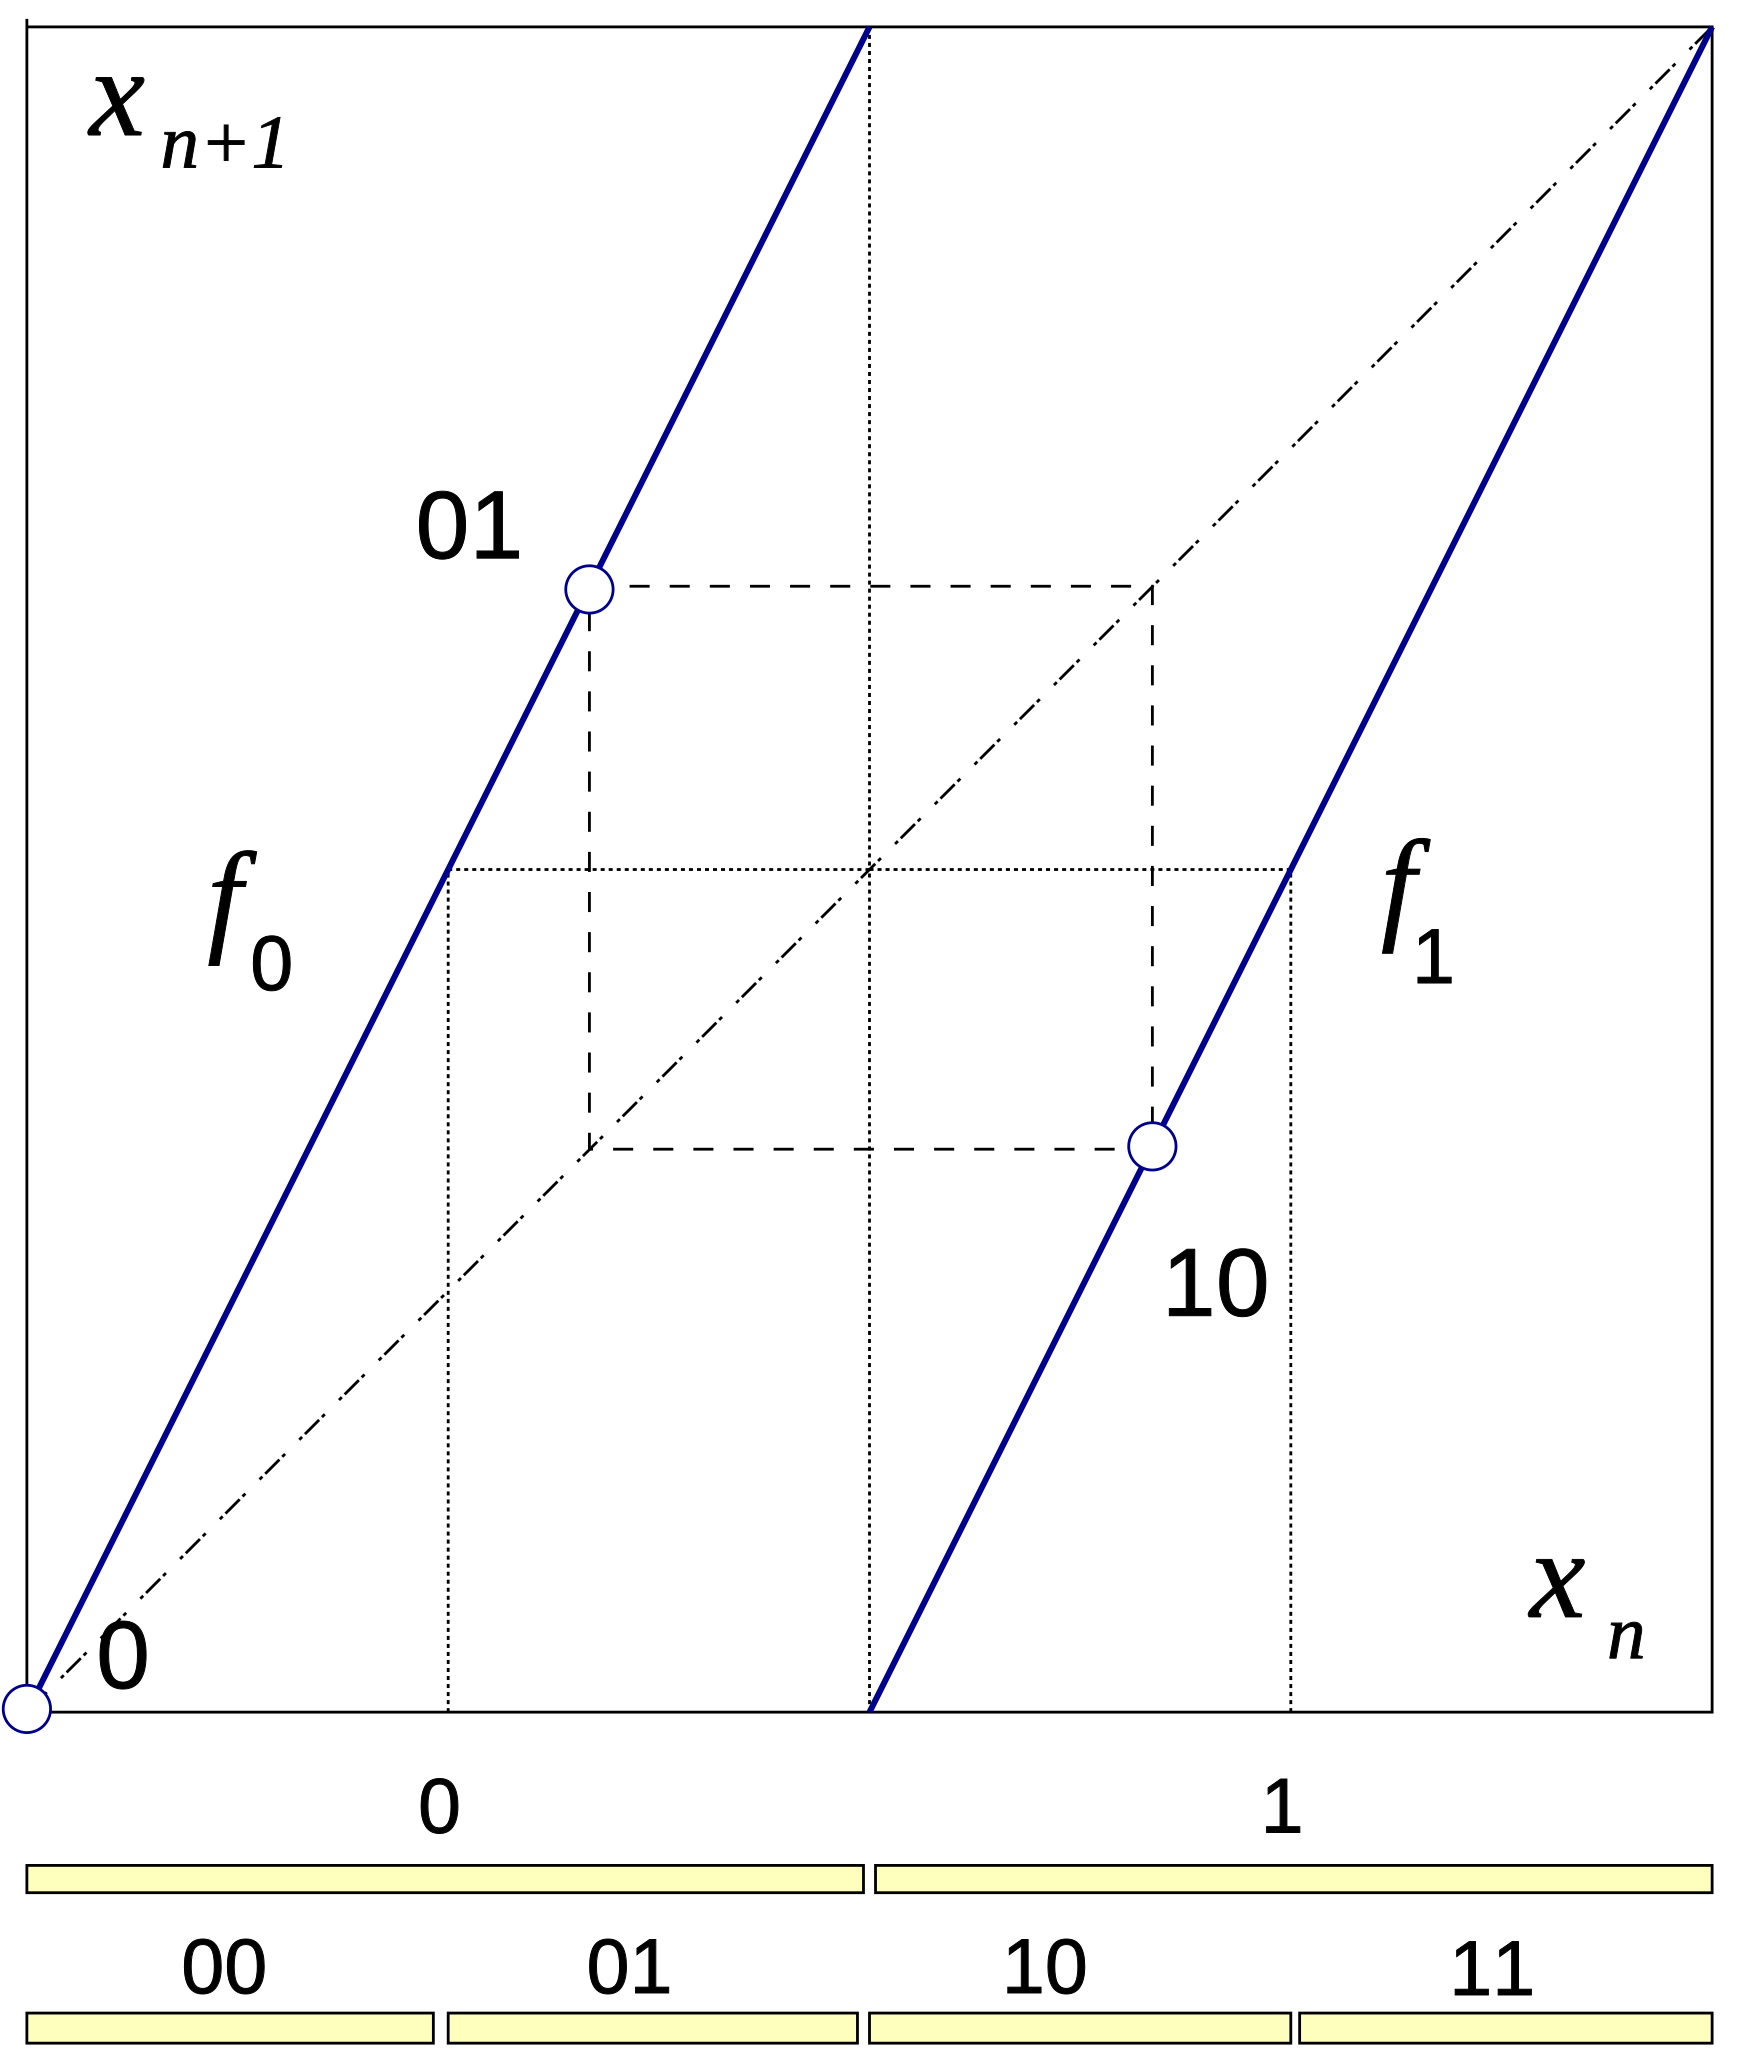
\includegraphics[width=0.35\textwidth]{BernPartCL18}
~~~
{(b)}$\!\!\!\!$
\includegraphics[width=0.40\textwidth]{fig_d_2CL18}

  \caption{\label{fig:BernPart}
(a)
The `coin toss' map \refeq{BerShift}, together with the
$\cycle{0}$ fixed point, and the \cycle{01} 2-cycle. Preimages
of the critical point $\ssp_c=1/2$ partition the unit interval into
$\{\pS_0,\pS_1\}$, $\{\pS_{00},\pS_{01},\pS_{10},\pS_{11}\}$, $\dots$,
subintervals.
(b)
The base-${s}$ Bernoulli map, here with the `dice throw' stretching parameter ${s}=6$,
partitions the unit interval into $6$ subintervals $\{\pS_{\Ssym{}}\}$,
labeled by the ${6}$-letter alphabet \refeq{base-sAlph}. As the map is a
circle map, $\ssp_{5}=1=0=\ssp_{0} \quad(\mbox{mod}\;1)$.
          }
\end{figure}
%%%%%%%%%%%%%%%%%%%%%%%%%%%%%%%%%%%%%%%%%%%%%%%%%%%%%%%%%%%%%%
%

The base-2 {\em Bernoulli} shift map,
\index{Bernoulli!shift}
\index{shift!Bernoulli}
\beq
\ssp_{\zeit+1} =
% \flow{}{\ssp_{\zeit}} =
\left\{ \begin{array}{ll}
        f_0(\ssp_{\zeit}) =  2 \ssp_{\zeit} \,, \quad
                                    & \ssp_{\zeit} \in \pS_0=[0,1/2) \\
        f_1(\ssp_{\zeit}) =  2 \ssp_{\zeit} \;\; (\mbox{mod}\;1)\,, \quad
                                    & \ssp_{\zeit} \in \pS_1 =[1/2,1)
         \end{array}\right.
\,,
\ee{BerShift}
is shown in \reffig{fig:BernPart}\,(a).
If the linear part of such map has an integer-valued slope,
or `stretching' parameter $s\geq2$,
\beq
\ssp_{\zeit+1} \,=\, {s} \ssp_{\zeit}
\ee{BerStretch}
that maps state $\ssp_{\zeit}$ into a state in the `extended \statesp',
outside the unit interval,
the $(\mbox{mod}\;1)$ operation results in the base-${s}$ Bernoulli
circle map,
\renewcommand{\ssp}{\ensuremath{\phi}}             % lattice site field
\beq
\ssp_{\zeit+1}
% = \flow{}{\ssp_{\zeit}}
= {s} \ssp_{\zeit}
\;\; (\mbox{mod}\;1)
%    \,,\qquad \qquad \ssp_{\zeit}\in [0,1)
\,,
\ee{n-tuplingMap}
sketched as a \HREF{https://www.random.org/dice/}{dice throw} in
\reffig{fig:BernPart}\,(b).
The $(\mbox{mod}\;1)$ operation subtracts
$\Ssym{\zeit+1}=\left\lfloor{s}\ssp_{\zeit}\right\rfloor$, the integer part of ${s}
\ssp_{\zeit}$, or the circle map \emph{winding number}, to keep
$\ssp_{\zeit+1}$ in the unit interval $[0,1)$, and partitions the unit
interval into ${s}$ subintervals $\{\pS_\Ssym{}\}$,
\beq
\ssp_{\zeit+1}
% = \flow{}{\ssp_{\zeit}}
% = \hflow{}{\ssp_{\zeit}} - \Ssym{\zeit+1}
= {s} \ssp_{\zeit} - \Ssym{\zeit+1}
\,,\qquad  \ssp_{\zeit}\in\pS_{\Ssym{\zeit}}
\,,
\ee{circ-m}
where $\Ssym{\zeit}$ takes values in the ${s}$-letter alphabet
\beq
\Ssym{} \in \A=\{0,1,2,\cdots,s-1\}
\,.
\ee{base-sAlph}

The Bernoulli map is a highly instructive example of a
hyperbolic dynamical system. Its symbolic dynamics is simple:
the base-${s}$ expansion of the initial point $\ssp_0$ is also its
temporal itinerary, with symbols from alphabet \refeq{base-sAlph}
indicating that at time $\zeit$ the orbit visits the subinterval
$\pS_{\Ssym{\zeit}}$. The map is a `shift':
a multiplication by ${s}$ acts on the base-${s}$
representation of $\ssp_{0}=.\Ssym{1}\Ssym{2}\Ssym{3}\cdots $ (for
example, binary, if ${s}=2$) by shifting its digits,
\bea
\ssp_{1}
    &=& \map(\ssp_{0})
    =.\Ssym{2}\Ssym{3}\cdots
%\continue
%\ssp_{\Ssym{2}\Ssym{3}\cdots}
%    &=& \shift{}\,\ssp_{\Ssym{1}\Ssym{2}\Ssym{3}\cdots}
\,.
\label{shiftBern}
\eea

Periodic points can be counted by observing that the preimages of
critical points $\{\ssp_{c1},\ssp_{c2},\cdots\ssp_{c,s-1}\}$ =
$\{{1}/s,{2}/s,\cdots,(s-1)/s\}$ partition the unit interval into
$\{\pS_0,\pS_1,\cdots,\pS_{s-1}\}$, $\{\pS_{\Ssym{1}\Ssym{2}}\}$, $\dots$,
$s^\cl{}$ subintervals, each containing {\em one}  unstable
period-$\cl{}$ periodic point
$\ssp_{\Ssym{1}\Ssym{2}\cdots\Ssym{\cl{}}}$, with stability multiplier
${s}^\cl{}$, see \reffig{fig:BernPart}. The Bernoulli map is a
full shift, in the sense that every itinerary is \admissible, with one
exception: on the circle, the rightmost fixed point is the same as the
fixed point at the origin, $\ssp_{s-1}=\ssp_{0}\quad(\mbox{mod}\;1)$,
so these fixed points are identified and counted as one, see
\reffig{fig:BernPart}. The total number of periodic points of period
$\cl{}$ is thus
\beq
N_{\cl{}} = s^{\cl{}} - 1
\,.
\ee{noPerPtsBm}


\subsection{Temporal Bernuolli}
\label{s:1D1dLatt}

To motivate our formulation of a \spt\ chaotic field theory to be
developed below, we now recast the local initial value, time-evolution
Bernoulli map problem as a \emph{temporal lattice} fixed point condition,
the problem of enumerating and determining all global solutions.

`Temporal' here refers to the state (field) $\ssp_\zeit$, and the winding
number (source) $\Ssym{\zeit}$ taking their values on the lattice sites
of a 1\dmn\ \emph{temporal} integer lattice $\zeit\in\integers$. Over a
finite lattice segment, these can be written compactly  as a
\emph{lattice state} and the corresponding \emph{symbol \brick}
\beq
\transp{\Xx} % = \{\ssp_j\}
             = (\ssp_{\zeit+1},\cdots,\ssp_{\zeit+\cl{}})
\,,\quad
\transp{\Mm} % = \{\Ssym{j}\}
             = (\Ssym{{\zeit+1}},\cdots,\Ssym{{\zeit+\cl{}}})
\,,
\ee{pathBern}
where $\transp{(\cdots)}$ denotes a transpose.
The Bernoulli equation \refeq{circ-m}, rewritten as a first-order
difference equation
\beq
\ssp_{\zeit} - {s}\ssp_{\zeit-1} = - \Ssym{\zeit}
\,,\qquad  \ssp_{\zeit} \in [0,1)
\,,
\ee{1stepDiffEq}
takes the matrix form
\beq
\jMorb\,\Xx = - \Mm
\,,\qquad
\jMorb = \id-{s}{\hopMat}^{-1}
% former \ee{tempBernFix}
\,,
\ee{tempBern}
where the $[\cl{}\!\times\!\cl{}]$ matrix
\beq
\hopMat_{jk}=\delta_{j+1,k}
\,,\qquad
\hopMat
=  \left(\begin{array}{ccccc}
             0    &  1    &        &   &  \cr
                  &  0    &   1    &   &  \cr
                  &       &        & \ddots &  \cr
                  &       &        & 0 & 1 \cr
             1    &       &        &   & 0
          \end{array} \right)
\,,
\ee{hopMatrix}
implements the shift operation \refeq{shiftBern}, a cyclic permutation
that translates forward in time the lattice state $\Xx$ by one site,
$\transp{(\hopMat \Xx)}=(\ssp_2,\ssp_3,\cdots,\ssp_\cl{},\ssp_1)$. The
time evolution law \refeq{circ-m} must be of the same form for all times,
so the {\shiftOp} $\hopMat$ has to be time-translation invariant, with
$\hopMat_{\cl{}+1,\cl{}}=\hopMat_{1\cl{}}=1$ matrix element enforcing the
periodicity. After $\cl{}$ shifts, a lattice state returns to the initial
state,
\beq
\hopMat^\cl{}=\id
\,.
\ee{shift2n}

As the {temporal Bernoulli} condition \refeq{tempBern} is a linear
relation, a given \brick\ $\Mm$, or `code' in terms of alphabet
\refeq{base-sAlph}, corresponds to a unique temporal lattice state $\Xx$.
That is why Percival and Vivaldi\rf{PerViv} refer to such symbol \brick\
$\Mm$ as a {\em linear code}.

\subsection{\JacobianOrb}
\label{s:JacobianOrb}

The {temporal lattice} reformulation gives us deep insights into how to
enumerate and determine all global solutions of such systems.
The {temporal Bernoulli} condition
\refeq{tempBern} can be viewed as a search for zeros of the function
\beq
F[\Xx] = \jMorb\Xx+\Mm = 0
\,,
\ee{tempFixPoint}
with the entire periodic \emph{lattice state} ${\Xx}_{\Mm}$ treated as a
single fixed \emph{point} $(\ssp_1,\ssp_{2},\cdots,\ssp_{\cl{}})$ in the
\cl{}\dmn\ \statesp\ unit hyper-cube $\Xx\in[0,1)^\cl{}$, where
the $[\cl{}\!\times\!\cl{}]$ matrix $\jMorb$ is given by \refeq{tempBern}.

The
$F[\Xx]=0$ fixed point condition \refeq{tempFixPoint} is central to the
theory of {global methods} for finding periodic orbits. Instead of
requiring forward-in-time numerical integrations, in multi-shooting
searches for \po s one discretizes a \po\ into $\cl{}$
segments\rf{auto,GM00aut,ChoGuck99,CvitLanCrete02,lanVar1,DingCvit14,DCTSCD14},
and lists a point for each segment
\beq
\transp{\Xx}=(\ssp_1,\ssp_2,\cdots,\ssp_\cl{})
\,.
\ee{nXdCycle}
Starting with an initial guess for \Xx, the zero of function
$F[\Xx]$ is then found by Newton iteration, which requires
an evaluation of the $[\cl{}\!\times\!\cl{}]$ \emph{\jacobianOrb}
\beq
\jMorb_{ij} =\frac{\delta F[\Xx]_i}{\delta \ssp_j}
\,.
\ee{jacobianOrb}

\subsection{Fundamental fact} %{Integer lattices}
\label{s:bernIntLat}

The {\jacobianOrb} \jMorb\ stretches the \statesp\ unit hyper-cube
$\Xx\in[0,1)^\cl{}$ into the \cl{}\dmn\ {\em \fundPip}, and maps each
periodic point ${\Xx}_{\Mm}$ into an integer lattice $\integers^\cl{}$
site, which is then translated by the winding numbers $\Mm$ into the
origin, in order to satisfy the fixed point condition
\refeq{tempFixPoint}. Hence $N_\cl{}$, the total number of the solutions
of the fixed point condition equals the number of integer lattice points
within the {\fundPip}, a number given by what Baake \etal\rf{BaHePl97}
call the \emph{`fundamental fact'},
\beq
N_\cl{} = |\Det\jMorb|
\,,
\ee{detBern0}
\ie, fact that the number of integer points in the {\fundPip} is equal to
its volume, or, what we refer to as the `{\HillDet}' below. In two
dimensions this formula is known since 1899 as
\HREF{https://en.wikipedia.org/wiki/Pick\%27s_theorem} {Pick's theorem},
in higher dimensions it was given by Nielsen\rf{Nielsen1920,BBPT75} in
1920, and rederived several times since in different contexts, for
example by Baake \etal\rf{BaHePl97}. For the task at hand,
Barvinok\rf{Barvinok04}
\HREF{http://www.math.lsa.umich.edu/~barvinok/lectures.pdf} {lectures}
offer a clear and simple introduction to integer lattices, and a proof of
\refeq{detBern0}.
% as {theorem 2}.

%%%%%%%%%%%%%%%%%%%%%%%%%%%%%%%%%%%%%%%%%%%%%%%%%%%%%%%%%%%%%%%%%%%%%%%
% BernCyc2Jacob.svg
% derived from CatMapStatesp.svg
\begin{figure}
  \centering
(a)~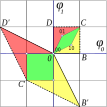
\includegraphics[width=0.35\textwidth]{BernCyc2JacobUnit}
~~~~~~
(b)~\includegraphics[width=0.22\textwidth]{BernCyc2JacobPart}
  \caption{\label{fig:BernCyc2Jacob}
  (a)
The Bernoulli map \refeq{BerShift} periodic points
$\Xx_\Mm=(\ssp_0,\ssp_1)$ of period 2 are the $\cycle{0}=(0,0)$ fixed
point, and the 2-cycle $\Xx_{01}=({1}/{3},{2}/{3})$, see
\reffig{fig:BernPart}\,(a). They all lie within the unit square $[0BCD]$,
which is mapped by the {\jacobianOrb} $\jMorb$ \refeq{bernFundPar} into
the {\fundPip} $[0B'C'D']$. Periodic points $\Xx_\Mm$ are mapped by
$\jMorb$ onto the integer lattice, $\jMorb\Xx_\Mm\in\integers^\cl{}$, and
are sent back into the origin by integer translations $\Mm$, in order to
satisfy the fixed point condition \refeq{tempFixPoint}. Note that this
{\fundPip} is covered by  3 unit area quadrilaterals, hence
$|\Det\jMorb|=3$.
    (b)
Conversely, in the flow conservation sum rule \refeq{H-OdeA_mapsOrb2} sum
over all lattice states $\Mm$ of period $\cl{}$, the inverse of the
{\HillDet} defines the `neighborhood' of a lattices state as the
corresponding fraction of the unit hypercube volume.
          }
\end{figure}
%%%%%%%%%%%%%%%%%%%%%%%%%%%%%%%%%%%%%%%%%%%%%%%%%%%%%%%%%%%%%%
%
The action of {\jacobianOrb}
$\jMorb$ for the period-2 lattice states (periodic points) of the Bernoulli map of
\reffig{fig:BernPart}\,(a), suffices to convey the idea. In this
case, the $[2\!\times\!2]$ {\jacobianOrb} \refeq{tempBern}, the unit
square basis vectors, and their images are
\bea
\jMorb &=&
 \left(\begin{array}{cc}
  1 & -2 \\
 -2 &  1
 \end{array} \right)
    \continue
\Xx^{(B)} &=&
 \left(\begin{array}{c}
 1  \\
 0
 \end{array} \right)
\;\to\;
\Xx^{(B')} = \jMorb\,\Xx^{(B)} =
 \left(\begin{array}{c}
  1  \\
 -2
 \end{array} \right)
\,,\quad \cdots
\nnu
\eea
\ie, the columns of the {\jacobianOrb} are the edges of the {\fundPip},
\beq
\jMorb = \left(\Xx^{(B')}\Xx^{(D')}\right)
\,,
\ee{bernFundPar}
see \reffig{fig:BernCyc2Jacob}\,(a), and $N_2=|\Det\jMorb|=3$,
in agreement with the periodic orbit count \refeq{noPerPtsBm}.

In general, the unit vectors of the \statesp\ unit hyper-cube
$\Xx\in[0,1)^\cl{}$ point along the \cl{} axes; {\jacobianOrb} \jMorb\
maps them into a {\fundPip} basis vectors $\Xx^{(j)}$, each one given by
a column of the $[\cl{}\!\times\!\cl{}]$ matrix
\beq
\jMorb = \left(\Xx^{(1)}\Xx^{(2)}\cdots\Xx^{(\cl{})}\right)
\,.
\ee{lattJac}
The {\HillDet} %discriminant
is then
\beq
\Det \jMorb = \Det\left(\Xx^{(1)}\Xx^{(2)}\cdots\Xx^{(\cl{})}\right)
\,,
\ee{lattVol}
the volume of the {\fundPip} whose edges are basis vectors $\Xx^{(j)}$.
Note that the unit hypercubes and {\fundPip}s are half-open, as indicated
by dashed lines in \reffig{fig:BernCyc2Jacob}\,(a), so that their translates
form a partition of the extended \statesp\ \refeq{BerStretch}.
For further examples of {\fundPip}s,
see \reffig{fig:catCycJacob} and \refeq{3times2basisVecs}.

Note that in the {temporal lattice} reformulation, the Bernoulli system
involves two distinct lattices:
\begin{itemize}
  \item[(i)]
In the latticization of the time continuum, one replaces \emph{any}
dynamical system's time-dependent field $\ssp(\zeit)\in\reals$ at time
$\zeit\in\reals$ by a discrete set of its values
$\ssp_\zeit=\ssp(\zeit\Delta{T})$ at time instants $\zeit\in\integers$.
Here the index $\zeit$ is a \emph{coordinate} over which the field
$\ssp$ is defined.
  \item[(ii)]
Specific to the Bernoulli system is the fact that the \emph{state}
$\ssp_{\zeit}$ \refeq{n-tuplingMap} is confined to the unit interval
$[0,1)$, imparting integer lattice structure onto the intermediate
calculational steps in the extended \statesp\ \refeq{BerStretch} on which
the {\jacobianOrb} \jMorb\ \refeq{tempBern} acts.
\end{itemize}


\subsection{Stability of an orbit vs. its time-evolution stability}
% maybe call this {Hill's formula for a general first-order system}
\label{s:notHill}   % was {exam:Hill1stOrd}
% siminos/spatiotemp/Examples/examHill1stOrd.tex

The {\jacobianOrb} $\jMorb_{ij}$ \refeq{jacobianOrb} is a high-\dmn\
linear stability matrix for a {\em zero} of function $F[\Xx]=0$,
evaluated on the lattice state $\Xx$. How is the stability so
computed related to the conventional dynamical systems, forward-in-time
stability? To motivate the answer, consider a temporal lattice with a set
of $d$ fields
$\ssp_{\zeit}=\{\ssp_{\zeit,1},\ssp_{\zeit,2},\dots,\ssp_{\zeit,d}\}$ on
each lattice site $\zeit$, and time evolution given by a $d$-\dmn\ map
$\ssp_{\zeit+1}=\map(\ssp_{\zeit})$.
An $\cl{}$-periodic lattice state $\Xx_p$ \refeq{pathBern} thus
% with $d$ fields
% $\ssp_{\zeit}=\{\ssp_{\zeit,1},\ssp_{\zeit,2},\dots,\ssp_{\zeit,d}\}$
% on each temporal lattice site $\zeit$
satisfies the first-order difference equation
\beq
\ssp_{\zeit} - \flow{}{\ssp_{\zeit-1}} = 0
    \,,\quad
\zeit=1,2,\cdots,\cl{}
\,.
\ee{1stepNonlimTemp}
A deviation $\Delta\Xx$ from $\Xx_p$ then satisfies the linearized condition
\beq
\Delta\ssp_{\zeit} - \jMat_{\zeit-1}\,\Delta\ssp_{\zeit-1} = 0
\,,\qquad
(\jMat_{\zeit})_{ij}
=
\left.\frac{\partial \flow{}{\ssp}_i}
           {\partial \ssp_{j}}\right|_{\ssp_{j}=\ssp_{\zeit,j}}
\,,
\ee{d-1stepJac2}
where $\jMat_{\zeit}$ is the 1-time step $[d\!\times\!{d}]$
\jacobianM.

It suffices to work out a temporal period $\cl{}=3$ example to understand
the calculation for any period. In terms of the $[3d\!\times\!3d]$
generalized \refeq{hopMatrix} shift matrix $\hopMat$, the \jacobianOrb\
\refeq{jacobianOrb} can be written in block matrix form
\beq
\jMorb_p \,=\,
\id - \hopMat^{-1} \jMat
\,,\quad
\hopMat^{-1} =
\left[
\begin{array}{ccc}
0     & 0     & \id_d  \\
\id_d & 0     & 0  \\
0     & \id_d & 0
\end{array}
\right]
\,,\quad
\jMat =
\left[
\begin{array}{ccc}
\jMat_1 & 0 & 0 \\
0 & \jMat_2 & 0  \\
0 & 0 & \jMat_3
\end{array}
\right]
\,,
\ee{3shift}
where $\id_d$ is the $d$-\dmn\ identity matrix.
Note that the third repeat of $\hopMat^{-1}\jMat$ is block-diagonal
\bea
(\hopMat^{-1}\jMat)^2 &=&
\hopMat^{-2}
\left[
\begin{array}{ccc}
\jMat_2\jMat_1 & 0 & 0 \\
0 & \jMat_3 \jMat_2 & 0  \\
0 & 0 & \jMat_1\jMat_3
\end{array}
\right]
,\;\;
(\hopMat^{-1}\jMat)^3  =
\left[
\begin{array}{ccc}
\jMat_2\jMat_1\jMat_3 & 0 & 0 \\
0 & \jMat_3\jMat_2\jMat_1 & 0  \\
0 & 0 & \jMat_1\jMat_3\jMat_2
\end{array}
\right],
\nnu %\label{stabSquare}
\eea
as $\hopMat^{-3}=\id$.
Likewise, as $\hopMat^\cl{}=\id$, the trace of the
$[\cl{}d\!\times\!\cl{}d]$ matrix for a period $\cl{}$ lattice state
\[
\Tr(\hopMat^{-1}\jMat)^k=\delta_{k,r\cl{}}\,\cl{}\,\tr\jMat_p^r
\,,\quad
\jMat_p = \jMat_\cl{}\jMat_{\cl{}-1}\cdots\jMat_2\jMat_1
\]
is non-vanishing only if $k$ is a multiple of $\cl{}$, where $\jMat_p$ is the
forward-in-time $[d\!\times\!{d}]$ Jacobian (or Floquet) matrix of the \po\ $p$.

Now we can evaluate the {\HillDet} $\Det(\jMorb_p)$ by expanding
\bea
\ln\Det(\jMorb_p) &=&
\Tr\ln(\id-{\hopMat}^{-1}\jMat)
                \,=\,
-\sum_{k=1}^\infty\frac{1}{k}\,\Tr({\hopMat}^{-1}\jMat)^k
    \continue
                 &=&
-\tr\sum_{r=1}^\infty\frac{1}{r} \jMat_p^{r}
  =
\ln\det(\id_d-\jMat_p)
\,.
\label{LnDet=TrLn2}
\eea
The {\jacobianOrb} $\jMorb_p$ evaluated on a lattice state $\Xx_p$
satisfying the temporal lattice first-order difference equation
\refeq{1stepNonlimTemp}, and the dynamical, forward in time \jacobianM\
$\jMat_p$ are thus related by \emph{Hill's formula}
\beq
\Det\jMorb_p = \det (\id_d-\jMat_p)
\,,
\ee{detDet}
which relates the global orbit stability to the Floquet, forward in time
evolution stability.
        \PC{2020-02-16}{Eventually drop this and
that section: ``
We work that out in detail in \refsect{s:HillForm}.
        ''
        }

For the particularly simple, linear {Bernoulli} case at hand,
the field $\ssp_\zeit$ is a scalar,
the 1-time step $[1\!\times\!1]$ time-evolution \jacobianM\
\refeq{d-1stepJac2} at every lattice point $\zeit$ is simply
$\jMat_{\zeit}={s}$,
and
the {\jacobianOrb}
\refeq{tempBern} is the same for all, in general
distinct lattice states of period $\cl{}$,
so
\beq
N_\cl{} = |\Det\jMorb| = {s}^{\cl{}} - 1
\,,
\ee{detBern2}
in agreement with the time-evolution count \refeq{noPerPtsBm}; all
itineraries are allowed, except that the periodicity of
$\hopMat^\cl{}=\id$ accounts for $\cycle{0}$ and
$\cycle{s\!-\!1}$ fixed points (see \reffig{fig:BernPart}) being a
single periodic point.



\subsection{\Po\ theory}
\label{s:PoThe}

How come that a `$\Det$' in \refeq{detBern0} counts lattice states?

For a general, nonlinear fixed point condition $F[\Xx]=0$, expansion
\refeq{LnDet=TrLn2} in terms of traces is a cycle
expansion\rf{inv,AACI,ChaosBook}, with support on \emph{periodic orbits}.
Ozorio de Almeida and Hannay\rf{OzoHan84} were the first to relate the
number of periodic points to a \JacobianM\ generated volume; in 1984 they
used such relation as an illustration of their `principle of uniformity':
``periodic points of an ergodic system, counted with their natural
weighting, are uniformly dense in phase space.'' In \po\
theory\rf{inv,CBgetused} this principle is stated as a
\HREF{http://chaosbook.org/chapters/ChaosBook.pdf\#section.27.4} {flow
conservation} sum rule, where the sum is over all lattice states $\Mm$ of
period $\cl{}$,
\beq
\sum_{|\Mm|=\cl{}}
    \frac{1}{|\det (\id - \jMat_\Mm)|}
    \;= 1
\,,
\label{H-OdeA_mapsOrb}
\eeq
or, by Hill's formula \refeq{detDet},
\beq
\sum_{|\Mm|=\cl{}}
%\sum_{\ssp_i{\in\mbox{\footnotesize Fix}\map^{\cl{}}}}
    \frac{1}{|\Det\jMorb_\Mm|}
    \;=1
\,.
\label{Det(jMorb)eights}
\eeq
For the Bernoulli system the `natural weighting' takes a particularly
simple form, as the {\HillDet} of the {\jacobianOrb} is the same for all
periodic points of period $\cl{}$, $\Det\jMorb_\Mm=\Det\jMorb$, whose
number is thus given by \refeq{detBern0}.
For example, the sum over the $\cl{}=2$ lattice states is,
\beq
      \frac{1}{|\Det{\color{green}\jMorb_{00}}|}
   +    \frac{1}{|\Det{\color{red}\jMorb_{01}}|}
   + \frac{1}{|\Det{\color{yellow}\jMorb_{10}}|}
    =1
\,,
\ee{H-OdeA_mapsOrb2}
see \reffig{fig:BernCyc2Jacob}\,(b).
Furthermore, for any piece-wise
linear system all curvature corrections\rf{CBcount} for orbits of
periods $k>\cl{}$ vanish, leading to explicit lattice state-counting
formulas of kind reported in this paper.

\subsection{Shadowing}
\label{s:bernShadow}
%        \PC{2020-01-30}{
% link to \templatt\ Green's function \refeq{1dLatGreenFct}
%        }

As the {temporal Bernoulli} condition \refeq{tempBern} is a linear
relation, a given \brick\ $\Mm$, or `code' in terms of alphabet
\refeq{base-sAlph}, corresponds to a unique temporal lattice state $\Xx$
given by the temporal lattice Green's function
\beq
\Xx_\Mm
= \gd\,\Mm
\,,\qquad
\gd = \frac{\hopMat/{s}}{\id- {\hopMat}/{s}}
\,.
\ee{tempBernGreen}
For an infinite lattice $\zeit\in\integers$, this Green's function can be
expanded as a series in $\ExpaEig^{-k}$,
\beq
\gd
    = \frac{\,{\hopMat}/{\ExpaEig}}{\id-{\hopMat/}{\ExpaEig}}
    = \sum_{k=1}^\infty \frac{\hopMat^k}{\ExpaEig^{k}}
\,,
\ee{BernGreenF}
where $\ExpaEig={s}$ is the 1-time step stability multiplier for the
Bernoulli system. From \refeq{tempBernGreen} it follows that
the influence of a source $\Ssym{\zeit'}$ back in the
past, at site $\zeit'$, falls off exponentially with the temporal lattice
distance $\zeit-\zeit'$,
\beq
  \ssp_{\zeit}=\sum_{\zeit'=-\infty}^{\zeit-1} g_{\zeit\zeit'} \Ssym{\zeit'}
\,, \quad
g_{\zeit\zeit'}
   =
   \frac{1}{\ExpaEig^{\zeit-\zeit'}}
\,,\quad \zeit>\zeit'\,,\quad  0\mbox{ otherwise}
\,.
\ee{BernGreenSites}
That means that an ergodic lattice state segment of length \cl{}\ (or a
periodic {lattice state} of a longer period) is shadowed by the periodic
{lattice state} \refeq{pathBern} with the same \cl{}-sites {symbol
\brick} $\Mm$,
    \PC{2020-02-16}{
Do I need to derive this?
    }
\beq
\ssp_{\zeit}
=  \frac{1}{1-1/\ExpaEig^{\cl{}}}
\left(\frac{\Ssym{1}}{\ExpaEig}+\frac{\Ssym{2}}{\ExpaEig^{2}}
      +\cdots
      +\frac{\Ssym{\cl{}-1}}{\ExpaEig^{\cl{}-1}}+\frac{\Ssym{\cl{}}}{\ExpaEig^{\cl{}}}
\right)
,
\label{Bern_cyc}
\eeq
with exponentially
decreasing shadowing error of order $O(1/\ExpaEig^{\cl{}+1})$. The error
is controlled by the \refeq{detDet} prefactor
\(
1/|\Det\jMorb| = 1/|\det(\id - \jMat_\Mm)|\,,
\)
with the determinant arising from inverting the {\jacobianOrb}
$\jMorb$ to obtain the Green's function \refeq{tempBern}.

This error estimate is deeper than what it might seem at the first
glance. In fluid dynamics, pattern recognition, neuroscience and other
high or $\infty$-dimensional settings distances between `close solutions'
(let's say pixel images of two faces in a face recognition code) are
almost always measured using some arbitrary yardstick, let's say a
Euclidean $L_2$ norm,
even though the state space that has no Euclidean symmetry.
Not so in the \po\ theory: here $1/|\Det\jMorb|$ is the \emph{intrinsic,
coordinatization and norm independent} measure of the distance between
similar \spt\ states.

\subsection{\Tzeta}
\label{s:bernZeta}

Now that we have the numbers of lattice states $N_{\cl{}}$ for any
period $\cl{}$, we can combine them all into a single generating function by
substituting $N_{\cl{}}$ into the {\em topological} or {\em Artin-Mazur}
zeta func\-tion\rf{ArtMaz65,CBcount},
\index{topological!zeta function}
\index{zeta function!topological}
\index{Artin-Mazur zeta function}
\index{zeta function!Artin-Mazur}
    \PC{2020-02-16}{
Do I need to derive this, rather than refer to ChaosBook?
    }
\beq
\zetatop(z) =
     \exp\left(-\sum_{\cl{}=1}^\infty
\frac{z^\cl{}}{\cl{}} N_\cl{}
         \right)
\,,
\ee{topoZeta}
which, when expanded as a Taylor series in $z$, is built from
\emph{primitive} (or \emph{prime}), \ie, non-repeating lattice
states\rf{inv}. Conversely, given the \tzeta, the number of periodic
points of period $\cl{}$ is given by the logarithmic derivative of the
{\tzeta} (see
\HREF{http://chaosbook.org/chapters/ChaosBook.pdf\#section.18.7}
{ChaosBook}\rf{CBcount})
\bea
\sum_{\cl{}=1}N_\cl{} z^\cl{}
    &=& - \,\frac{1}{\zetatop}\,z\frac {d}{dz} (\zetatop)
\,.
\label{zetatop-N}
\eea

For a Bernoulli system \refeq{detBern2},
\bea
\zetatop(z)
 &=&  \exp \left(-\sum_{\cl{}=1}^\infty
\frac{z^\cl{}}{\cl{}} ({s}^\cl{} - 1)
         \right)
\,=\,
\exp \left[\ln(1 -  {s}z) - \ln(1 - z) \right]
\continue
 &=&
\frac{1 -  {s}z}{1 - z}
\,.
\label{BernZeta}
\eea
The numerator $(1 - {s}z)$ says that a Bernoulli system is a full
shift\rf{CBcount}: there are $s$ fundamental lattice states, in this case
fixed points $\{\ssp_0,\ssp_1,\cdots,\ssp_{s-1}\}$, and every other
lattice state is built from their concatenations and repeats. The
denominator $(1 - z)$ compensates for the single overcounted lattice
state, the fixed point $\ssp_{{s}-1}=\ssp_{0}$ $(\mbox{mod}\;1)$ of
\reffig{fig:BernPart} and its repeats.

\subsection{Counting {temporal Bernoulli} prime \po s}
\label{s:bernPrime}

Substituting the Bernoulli map \tzeta\ \refeq{BernZeta}
into \refeq{zetatop-N}
we obtain
% ------------------- siminos/mathematica/ ----------
% CatMaptopZeta.nb                                    2020-01-18
% Bernoulli map periodic points counting for CL18.tex
\bea
\sum_{n=1}N_n z^n
    &=&
 z+3 z^2+7 z^3+15 z^4+31 z^5+63 z^6+127 z^7
    \ceq
+255 z^8+511 z^9+ 1023z^{10} +2047 z^{11}
\cdots
\,,
\label{bernN_n-s=2}
\eea
in agreement with the lattice states count \refeq{detBern2}.
The number of \emph{prime} cycles of period $\cl{}$ is given recursively by
subtracting repeats of shorter prime cycles\rf{CBcount},
\beq
M_n\,=\,\frac{1}{n}\left( N_n - \sum _{d|n}^{d<n}\,d M_d \right)
\,,
\ee{primeCount}
where $d$'s are all divisors of $n$, hence
% ------------------- siminos/mathematica/ ----------
% CatMaptopZeta.nb                                    2020-01-18
% Bernoulli map periodic points counting for CL18.tex
\bea
\sum_{n=1}M_n z^n
    &=&
 z+  z^2+2 z^3+3 z^4+6 z^5+9 z^6+18 z^7
    \ceq
+30 z^8+56 z^9+99 z^{10} +186 z^{11}
\cdots
\,,
\label{bernM_n-s=2}
\eea
in agreement with the usual numbers of binary symbolic dynamics prime
cycles\rf{CBcount}.

\subsection{Bernoulli as a continuous time dynamical system}
\label{s:bernODE}

The discrete time derivative of a lattice state \Xx\ evaluated at the
lattice site \zeit\ is given by the \emph{difference operator}\rf{Elaydi05}
    \index{lattice!derivative}\index{derivative, lattice}
    \index{lattice!derivative, forward}\index{difference operator}
\beq
\dot{\Xx}_\zeit =
\left[\frac{\partial\Xx}{\partial\zeit}\right]_\zeit
        =
    \frac{\ssp_{\zeit} - \ssp_{\zeit-1}}{\Delta\zeit}
\ee{lattTimeDer}
The {temporal Bernoulli} condition \refeq{1stepDiffEq} can be thus viewed
as a time-discretized, first-order ODE dynamical system
\beq
   \dot{\Xx} \,=\, \vel(\Xx) \,,
\ee{1stepVecEq}
where the `velocity' vector field $\vel$ is given by
\[
\vel(\Xx) \,=\,
   % \vel(\Xx;\Mm) \,=\,
(s-1)\,\hopMat^{-1}\,\Xx-\Mm
\,,
\]
with the time increment set to $\Delta\zeit=1$, and perturbations that
decay (or grow) with rate $({s}-1)$. By inspection of
\reffig{fig:BernPart}\,(a), it is clear that for \emph{shrinking},
${s}<1$  parameter values the orbit is stable forward in time, with a
single linear branch, 1-letter alphabet $\A=\{0\}$, and the only periodic
lattice states being the single fixed point  $\ssp_0=0$, and its repeats
$\Xx=(0,0,\cdots,0)$. However, for \emph{stretching},  ${s}>1$  parameter
values Bernoulli systems that we study here, every periodic lattice state
$\Xx_\Mm$ is unstable, and there is a \po\ solution for each symbol
\brick\ \Mm.

As far as the time-evolution stability is concerned, the
$|\Det\jMorb_\Mm|=|\det (\id-\jMat_\Mm)|$ formula \refeq{detDet} is
correct for all first-order difference equations (systems whose evolution
laws are first order in time), for any $[d\times{d}]$ one-time-step
{\jacobianM}. For the Bernoulli system that is a $[1\!\times\!1]$ matrix
$\jMat=s$, with the periodic points count \refeq{detBern2} trivially
verified.

The {\jacobianOrb} %\refeq{1stepVecEq},
$\jMorb=\partial/\partial\zeit-(s-1)\,\hopMat^{-1}$ is a differential
operator whose determinant one usually computes by a Fourier transform
diagonalization (see \refappe{appe:Fourier}). The Fourier discretization
approach goes all the way back to Hill's 1886 paper\rf{Hill86}; in the
limit of $\cl{}\to\infty$ multi-shooting steps \refeq{nXdCycle}, this is
a remarkable formula, relating a field-theoretic, $\infty$\dmn\
\emph{functional} {\HillDet} $\Det\jMorb_\Mm$ to a determinant of the
finite, $[d\times{d}]$ matrix $\jMat_\Mm$, and it took
\Poincare\rf{Poinc1886} to prove that Hill's Fourier modes calculation is
correct in the continuum limit. Historically,  in \po\ theory
calculations one always computes $\jMat_\Mm$. However, as we shall show
here, and in more generality in \refsect{s:Hill}, it is the {\HillDet}
$\Det\jMorb$ that is the computationally robust quantity that one should
evaluate.

\bigskip

\noindent\textbf{A fair coin toss, summarized.}
We refer to the \emph{global} temporal lattice condition \refeq{tempBern}
as the `\emph{temporal} Bernoulli', in order to distinguish it from the
one-time step Bernoulli evolution \emph{map} \refeq{n-tuplingMap}, in
preparation for the study of \emph{\spt} systems to be undertaken in
\refsect{s:catlatt}. In the lattice formulation, a \emph{global}
{temporally periodic lattice state} $\Xx_\Mm$ is determined by the
requirement that the \emph{local} temporal lattice condition
\refeq{1stepDiffEq} is satisfied at every lattice site. For {temporal
Bernoulli} there is no need for forward-in-time searches for the
returning periodic points. Instead, one determines each global
{temporally periodic lattice state} $\Xx_\Mm$ at one go, by solving the
fixed point condition \refeq{tempFixPoint}, and one determines the total
number of lattice states by computing the {\HillDet} \refeq{detBern0} of
the \emph{\jacobianOrb}. The most importantly for what follows, this
calculation requires no recourse to any \emph{explicit coordinatization
of system's state space} (as, for example, the \AW\ partition),
    \PC{2020-12-17}{
Link to the ChaosBook.
    }
and \emph{no explicit symbolic dynamics}.
This is the `\po\ theory'. And if you don't know,
\HREF{https://www.youtube.com/watch?v=_JZom_gVfuw} {now you know}.

The observation that a Bernoulli system can be viewed as a discretization
of a first-order in time ODE, eq.~\refeq{1stepVecEq}, with solutions
whose temporal global linear stability is described by the {\jacobianOrb}
$\jMorb_{ij}=\delta{F[\Xx]}_i/\delta\ssp_j$, has profound implications
for dissipative \spt\ systems such as Navier-Stokes and
Kuramoto-Sivashinsky\rf{GuBuCv17}. However, the goal here is to formulate
a classical {\spt}ly chaotic field theory, Hamiltonian and energy
conserving, because (a) that is physics, and (b) cannot do quantum theory
without it. We need a system as simple as the Bernoulli map, but
mechanical. So, we move on from running in circles, to a mechanical rotor
to kick.

%%%%%%%%%%%%%%%%%%%%%%%%%%%%%%%%%%%%%%%%%%%%%%%%%%%%%%%%%%%%%%%%%%%%%%%
\renewcommand{\statesp}{phase space}
\renewcommand{\Statesp}{Phase space}
\renewcommand{\stateDsp}{phase-space}
\renewcommand{\StateDsp}{Phase-space}
